\documentclass[12pt,a4paper,notitlepage]{report}
\usepackage[utf8]{inputenc}
\usepackage{import}
\usepackage[english,french]{babel}
\usepackage{amsmath}
\usepackage{amsfonts}
\usepackage{amssymb}
\usepackage{graphicx}
%caption and reference
\usepackage{caption}
\usepackage{subcaption}
\usepackage{hyperref}
%defaut image path
\graphicspath{ {image/} }
%fixme note
\usepackage[nomargin,inline,marginclue,draft]{fixme}
%line spacing and first paragraph indent
\usepackage[left=2cm,right=2cm,top=2cm,bottom=2cm]{geometry}
\setlength{\parskip}{1em}
%for table
\usepackage{multirow}
%Continuous 
\usepackage{chngcntr}
\counterwithout{figure}{chapter}

%for pseudocode
\usepackage{algorithm}
\usepackage[noend]{algpseudocode}
\makeatletter
\def\BState{\State\hskip-\ALG@thistlm}
\makeatother
\usepackage{indentfirst}
\usepackage{pdfpages}
\usepackage{tikz}
\usetikzlibrary{shapes,arrows}
% styles for flowcharts
\tikzstyle{block} = [rectangle, draw, text width=10em, text centered, rounded corners, minimum height=4em,fill=blue!20]
\tikzstyle{cloud} = [draw, ellipse,fill=red!20, node distance=3cm,
minimum height=2em]
\author{HUYNH Le Duy}

%Color
\usepackage{xcolor}
\usepackage{sectsty}
\definecolor{TB}{RGB}{189,190,0}
\chapterfont{\color{TB}}  % sets colour of chapters



\begin{document}
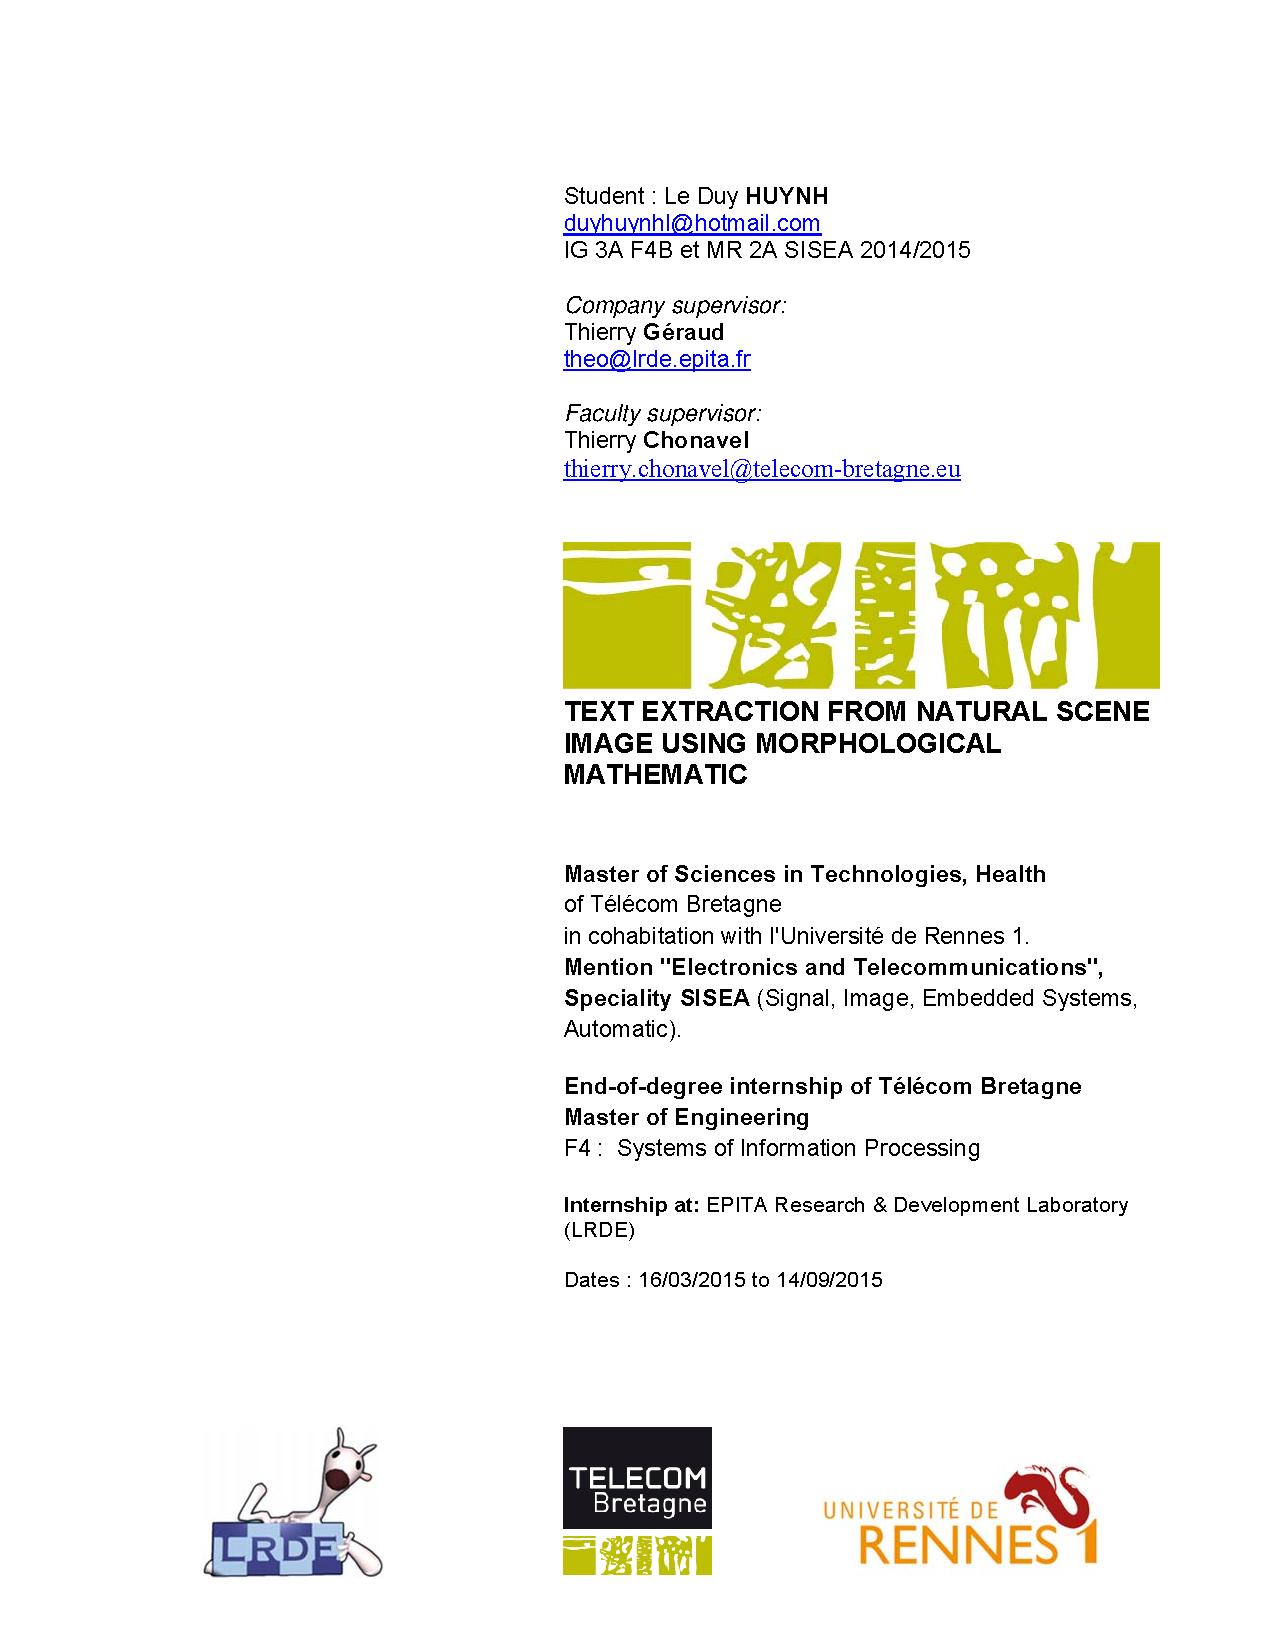
\includepdf{0TitlePage/title}
\import{0TitlePage/}{title}
\tableofcontents
\listoffigures
\import{1chapterIntroduction/}{chapterIntroduction}
\import{2chapterStateOfArt/}{chapterStateOfArt}
\import{3chapterTheory/}{chapterTheory}
\import{4chapterOurApproach/}{ourApproach}
\import{5chapterImplementation/}{implementation}
\import{6chapterExperimental/}{Experimental}
\import{7chapterConclusion/}{Conclusion}

\bibliographystyle{plain}
\bibliography{Reference/bibli}

\end{document}

%seem good on chromatics